\chapter{Menyiapkan Lingkungan Pengembangan (Dev Environment)}
\label{chap:python_setup}

Untuk benar-benar menguasai AI, Anda harus berani menyentuh sedikit kode. Bahasa pemrograman standar untuk AI adalah **Python**. Jangan khawatir, Python sangat mirip dengan bahasa Inggris.

\section{Langkah 1: Instalasi Python}

\begin{center}
    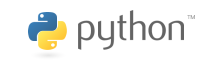
\includegraphics[width=0.4\textwidth]{ai_literacy_guide/images/python-logo.png}
\end{center}

\begin{enumerate}
    \item Buka website resmi \url{https://www.python.org/downloads/}.
    \item Download versi terbaru (minimal 3.10 ke atas).
    \item \textbf{PENTING:} Saat instalasi, centang kotak \textbf{"Add Python to PATH"}. Jika ini terlewat, komputer Anda tidak akan mengenali perintah Python.
    \item Selesaikan instalasi.
\end{enumerate}

\section{Langkah 2: Instalasi VS Code}

Kita butuh editor teks yang canggih. VS Code adalah standar industri.

\begin{enumerate}
    \item Download di \url{https://code.visualstudio.com/}.
    \item Install seperti biasa.
    \item Buka VS Code, lalu klik menu "Extensions" (ikon kotak-kotak di kiri).
    \item Cari dan install ekstensi "Python" dari Microsoft.
\end{enumerate}

\section{Langkah 3: Virtual Environment (Venv)}

Dalam proyek AI, library sering bentrok satu sama lain. Kita menggunakan "Virtual Environment" untuk mengisolasi setiap proyek.

\begin{codeblock}[title=Membuat Venv di Terminal]
# 1. Buat folder proyek
mkdir proyek_ai_pertama
cd proyek_ai_pertama

# 2. Buat virtual environment
python -m venv venv

# 3. Aktifkan venv
# Windows:
venv\Scripts\activate
# Mac/Linux:
source venv/bin/activate
\end{codeblock}

Jika berhasil, Anda akan melihat tanda `(venv)` di sebelah kiri baris perintah Anda.

\section{Langkah 4: Menginstall Library AI}

Library adalah kumpulan kode yang sudah jadi. Untuk AI, kita butuh beberapa library utama.

\begin{codeblock}[title=Install Libraries]
pip install openai langchain python-dotenv notebook
\end{codeblock}

\begin{itemize}
    \item \textbf{openai:} Library resmi untuk mengakses GPT-4.
    \item \textbf{langchain:} Framework untuk membangun aplikasi AI kompleks.
    \item \textbf{python-dotenv:} Untuk mengelola API Key dengan aman.
    \item \textbf{notebook:} Untuk menjalankan Jupyter Notebook.
\end{itemize}

\section{Hello World: Skrip AI Pertama Anda}

Buat file baru bernama \texttt{hello\_ai.py} dan ketik kode berikut:

\begin{codeblock}[language=Python]
import os
from dotenv import load_dotenv

# Load API Key (nanti kita bahas cara dapatnya)
load_dotenv()

print("Lingkungan AI siap digunakan!")
\end{codeblock}

Jalankan dengan perintah:
\begin{codeblock}
python hello_ai.py
\end{codeblock}

Jika muncul tulisan "Lingkungan AI siap digunakan!", selamat! Anda sudah siap menjadi AI Engineer pemula.

\begin{exercisebox}
\textbf{Troubleshooting:}
Jika muncul error "pip is not recognized", artinya Anda lupa mencentang "Add Python to PATH". Uninstall Python dan install ulang dengan benar.
\end{exercisebox}
